% -*- compile-command: "make slides.pdf" -*-
\documentclass{beamer} 
\usepackage{tikz}
\usepackage[all]{xy}
\usepackage{amsmath,amssymb}
\usepackage{hyperref}
\usepackage{graphicx}
\usepackage{algorithmic}
\usepackage{multirow}

\usepackage[utf8]{inputenc}%for french accents. 
%\usepackage{appendixnumberbeamer}

\addtobeamertemplate{navigation symbols}{}{%
    \usebeamerfont{footline}%
    \usebeamercolor[fg]{footline}%
    \hspace{1em}%
    \insertframenumber/\inserttotalframenumber
}

\DeclareMathOperator*{\argmin}{arg\,min}
\DeclareMathOperator*{\Lik}{Lik}
\DeclareMathOperator*{\Peaks}{Peaks}
\DeclareMathOperator*{\Segments}{Segments}
\DeclareMathOperator*{\argmax}{arg\,max}
\DeclareMathOperator*{\maximize}{maximize}
\DeclareMathOperator*{\minimize}{minimize}
\newcommand{\sign}{\operatorname{sign}}
\newcommand{\RR}{\mathbb R}
\newcommand{\ZZ}{\mathbb Z}
\newcommand{\NN}{\mathbb N}
\definecolor{pDPA}{HTML}{1B9E77}
\definecolor{PELT}{HTML}{D95F02}
\definecolor{FPOP}{HTML}{7570B3}
\newcommand{\algo}[1]{\textcolor{#1}{#1}}
\definecolor{PDPA}{HTML}{66C2A5}
\definecolor{CDPA}{HTML}{FC8D62}
\definecolor{GPDPA}{HTML}{4D4D4D}




% Set transparency of non-highlighted sections in the table of
% contents slide.
\setbeamertemplate{section in toc shaded}[default][100]
\AtBeginSection[]
{
  \setbeamercolor{section in toc}{fg=red} 
  \setbeamercolor{section in toc shaded}{fg=black} 
  \begin{frame}
    \tableofcontents[currentsection]
  \end{frame}
}

\begin{document}

\title{CS599\\Machine Learning Research
\\Lecture 1: applications of machine learning}
  \date{27 August 2019}
\author{
  Toby Dylan Hocking\\
  toby.hocking@nau.edu
}

%To open: syllabus, google translate, mp3 player.

\maketitle

% \begin{frame}
%   \frametitle{Toby Dylan Hocking, brief CV}
%   \begin{description}
%   \item[2002-2006] UC Berkeley, double major in Molecular Cell Biology
%     and Statistics (honors thesis with Terry Speed).
%   \item[2006-2008] Biochemistry (DNA-binding specificity of zinc
%     finger proteins) and statistics at Sangamo BioSciences.
%   \item[2008-2009] Masters in Statistics, Paris 6.
%   \item[2009-2012] PhD in Mathematics from Ecole Normale Superieure de
%     Cachan, machine learning for cancer genomics with JP Vert (Inst Curie)
%     and Francis Bach (INRIA).
%   \item[2013] Postdoc in Computer Science (machine learning) with Masashi Sugiyama at Tokyo
%     Institute of Technology.
%   \item[2014-2017] Postdoc on machine learning for epigenomics
%     at McGill with Guillaume Bourque.
%   \end{description}
% \end{frame}

% \section{Introduction to machine learning}

\begin{frame}
  \frametitle{Machine learning intro: image classification example}
  ML is all about learning predictive functions $f(x)\approx y$, where 
  \begin{itemize}
  \item Inputs/features $x$ can be easily computed using traditional
    algorithms, e.g. matrix of pixel intensities in an image.
  \item Outputs/labels $y$ are what we want to predict, easy to get by
    asking a human, but hard to compute using traditional algorithms,
    e.g. image class.
  \item Input $x$ = image of digit, output $y\in\{0,1,\dots,9\}$, \\--
    this is a classification problem with 10 classes.\\
  $f(
\includegraphics[height=1cm]{mnist-0})=0$,
  $f(
\includegraphics[height=1cm]{mnist-1})=1$
\item Traditional/unsupervised algorithm: I give you a pixel intensity matrix
  $x\in\RR^{16\times 16}$, you code a function $f$ that returns one of
  the 10 possible digits. Q: how to do that?
  \end{itemize}
\end{frame}

\begin{frame}
  \frametitle{Supervised machine learning algorithms}

  I give you a training data set with paired inputs/outputs, e.g.

  \begin{center}
    \Huge 0 1 2 3 4 5 6 7 8 9

  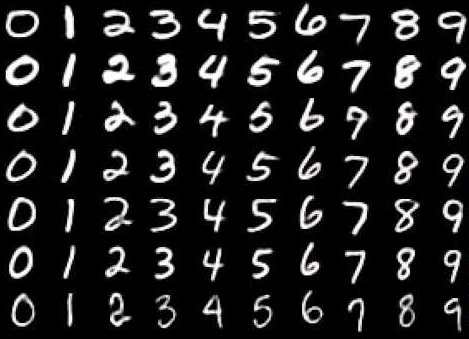
\includegraphics[height=1.9in]{mnist-digits}
  \end{center}

  Your job is to code an algorithm that learns the function $f$ from
  the training data. (you don't code $f$)
  
  \scriptsize Source: github.com/cazala/mnist
\end{frame}

\begin{frame}
  \frametitle{Supervised machine learning algorithms}

  \textbf{Can} be used typically whenever a knowledgeable/skilled
  human can easily/quickly/consistently create a large database of
  labels.

  \vskip 1in

  \textbf{Should} be used if it is not easy to code the function $f$
  for predicting the labels by hand.

\end{frame}



\begin{frame}
  \frametitle{Advantages of supervised machine learning}

  \begin{center}
      \begin{tabular}{cc}
        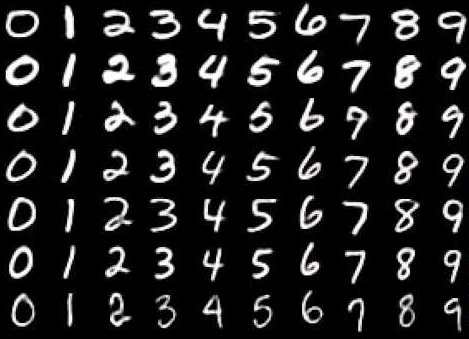
\includegraphics[height=1.5in]{mnist-digits} &
  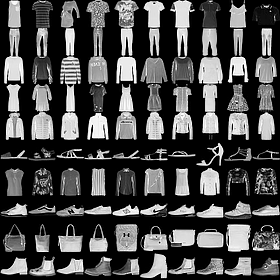
\includegraphics[height=1.5in]{fashion-mnist-sprite-some}  
  \end{tabular}
  \end{center}
  \vskip -0.2cm
  
  \begin{itemize}
  \item Input $x\in\RR^{16\times 16}$, output $y\in\{0,1,\dots,9\}$ types the same!
  \item Can use same learning algorithm regardless of pattern.
  \item Pattern encoded in the labels (not the algorithm).
  \item Useful if there are many un-labeled data, but few labeled data
    (or getting labels is long/costly).
  \item State-of-the-art accuracy (if there is enough training data).
  \end{itemize}

  \scriptsize Sources: github.com/cazala/mnist, github.com/zalandoresearch/fashion-mnist

\end{frame}

\begin{frame}
  \frametitle{Learning two different functions}
  Say \textsc{Learn} is a learning algorithm you have coded.
  \begin{center}
      \begin{tabular}{c}
        \textsc{Learn}(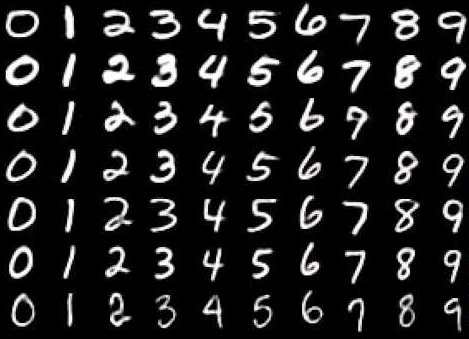
\includegraphics[height=1in]{mnist-digits}) $\rightarrow f$, 
        \textsc{Learn}(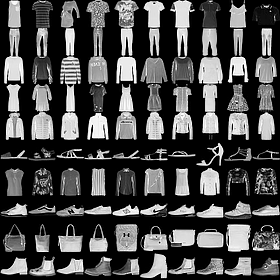
\includegraphics[height=1in]{fashion-mnist-sprite-some}) $\rightarrow g$
  \end{tabular}
  \end{center}
  \begin{itemize}
  \item Then we would expect
    $f(
\includegraphics[height=1cm]{mnist-0})=0$,
    $f(
\includegraphics[height=1cm]{mnist-1})=1$
  \item $g(
\includegraphics[height=1cm]{fashion-mnist-boot})=\text{shoe/0}$,
  $g(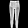
\includegraphics[height=1cm]{fashion-mnist-pants})=\text{pants/1}$
  \item Q: what happens if you do 
    $f(
\includegraphics[height=1cm]{fashion-mnist-boot})$, or
   $g(
\includegraphics[height=1cm]{mnist-0})$?

  \end{itemize}
\end{frame}

\begin{frame}
  \frametitle{Machine learning for cell image classification (CellProfiler)}
  Jones {\it et al.} PNAS 2009. Scoring diverse cellular morphologies in
  image-based screens with iterative feedback and machine learning.

\parbox{2in}{
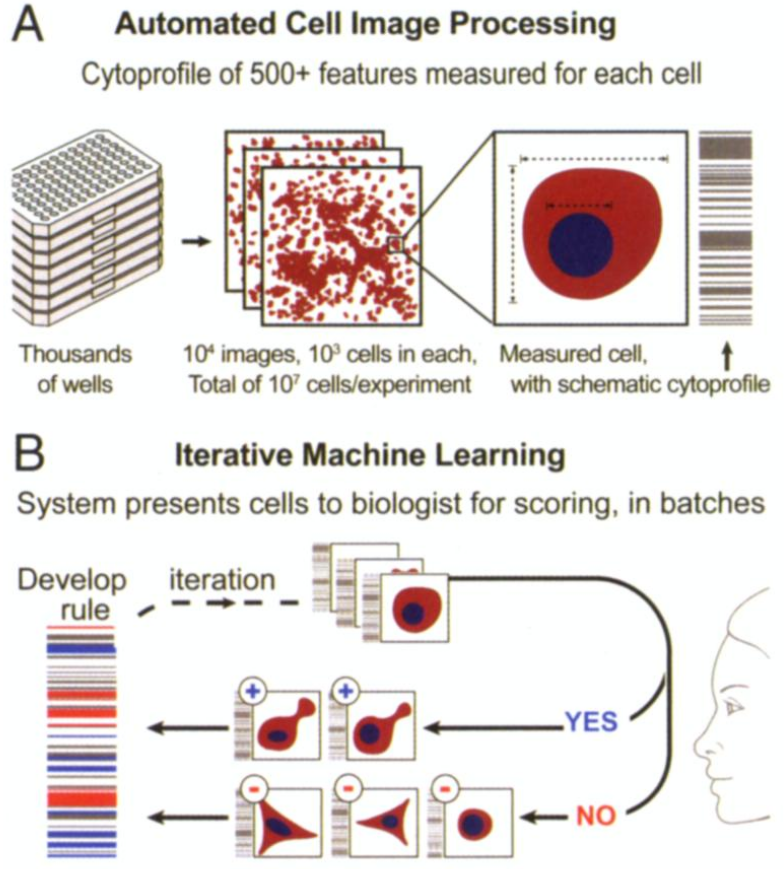
\includegraphics[width=2in]{cellprofiler} 
}
\parbox{2in}{
\begin{itemize}
  \item Input $x$ = image of cell, 
  \item Output $y\in\{\text{yes}, \text{no}\}$ (binary classification),
  \item $f(
\includegraphics[height=1cm]{cellprofiler-yes})=\text{yes}$,
  \item $f(
\includegraphics[height=1cm]{cellprofiler-no})=\text{no}$.
  \end{itemize}
}
\end{frame}

\begin{frame}
  \frametitle{Machine learning for image segmentation (LabelMe)}

  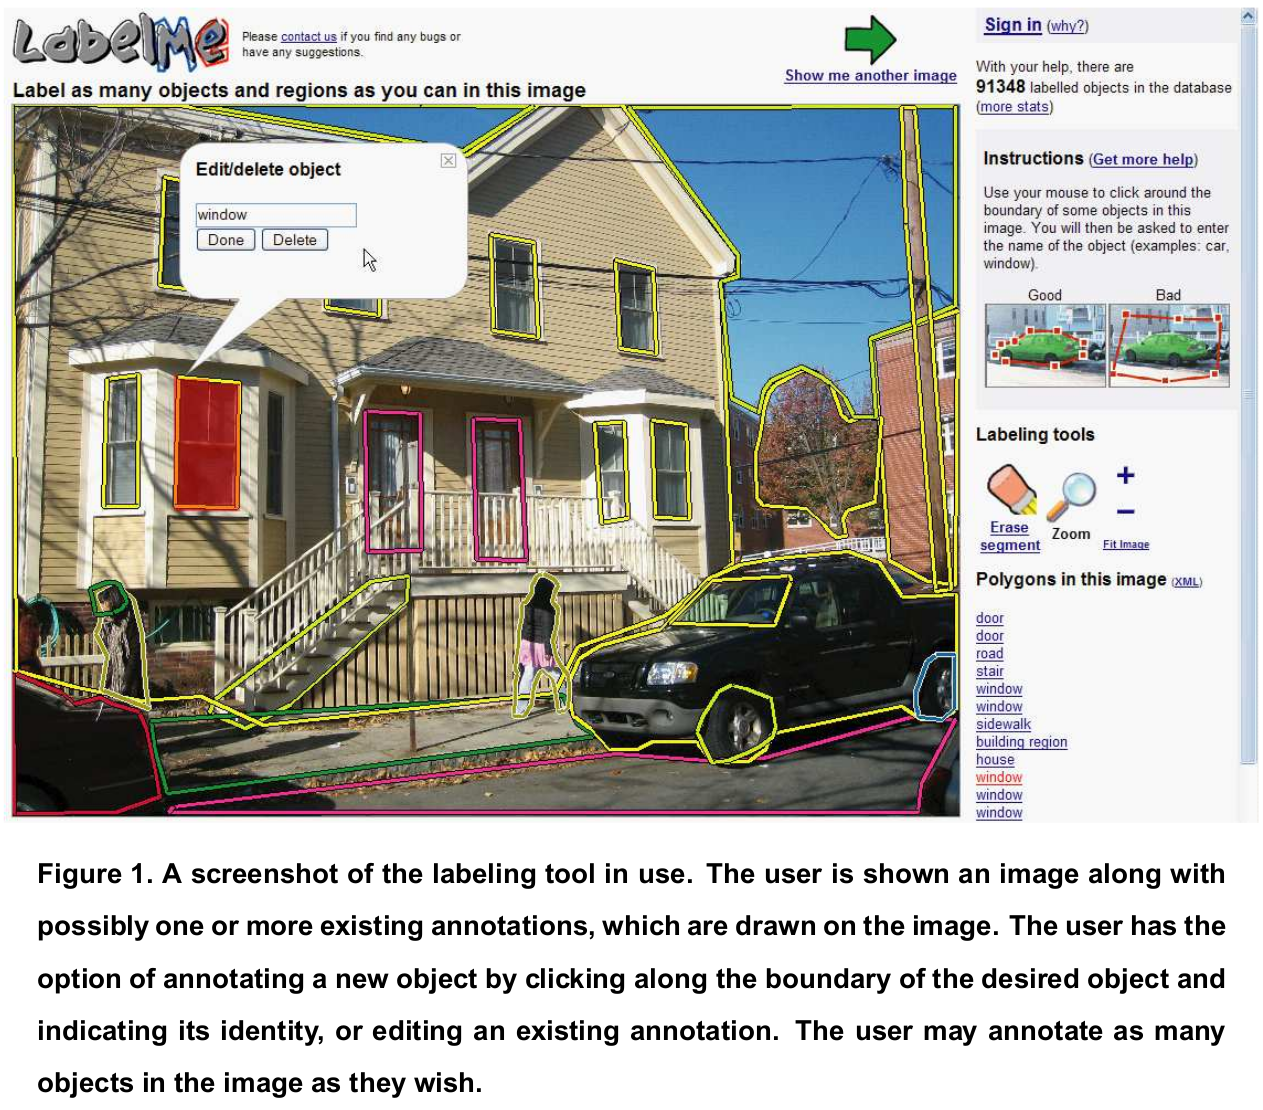
\includegraphics[width=\textwidth]{image-segmentation/labelme-interface}

\end{frame}

\begin{frame}
  \frametitle{Machine learning for image segmentation}

  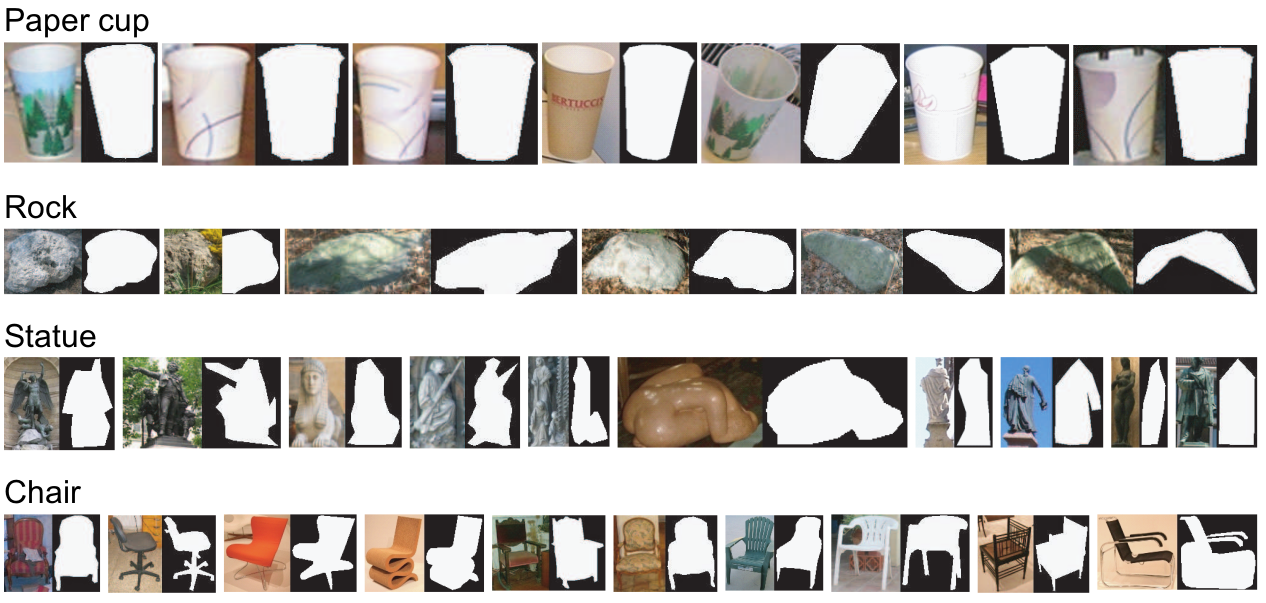
\includegraphics[width=\textwidth]{image-segmentation/labelme-examples}

  Russell {\it et al.} 2007.

  Q: What are the types/dimensions of $x,y,f$ in this example?

\end{frame}



\begin{frame}
  \frametitle{Machine learning for spam filtering (Gmail)}

  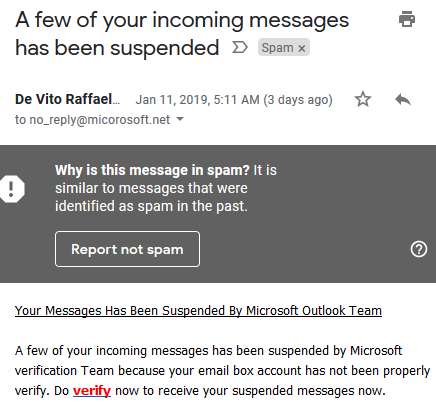
\includegraphics[height=2in]{spam-filtering/screenshot-gmail-spam}
  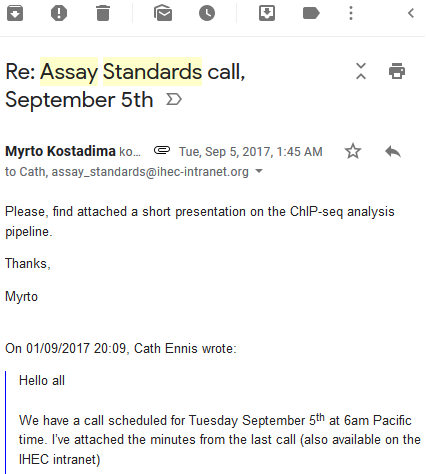
\includegraphics[height=2in]{spam-filtering/screenshot-inbox-message}

  Want: $f$(email message)$\in\{0,1\}$ -- binary classification, spam=1
  or not=0.

\end{frame}


\begin{frame}
  \frametitle{Machine learning for translation (google books)}

  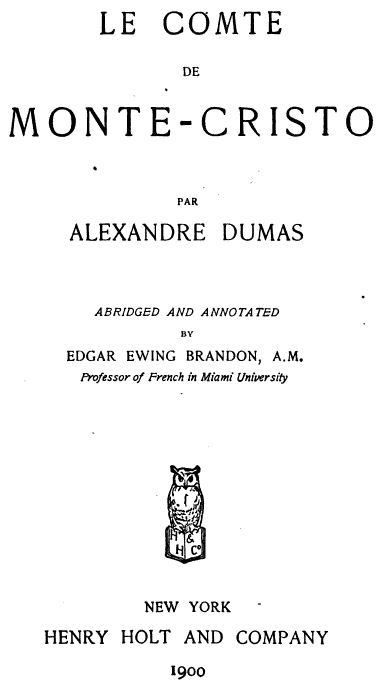
\includegraphics[height=3in]{translation/monte-cristo-french-title}
  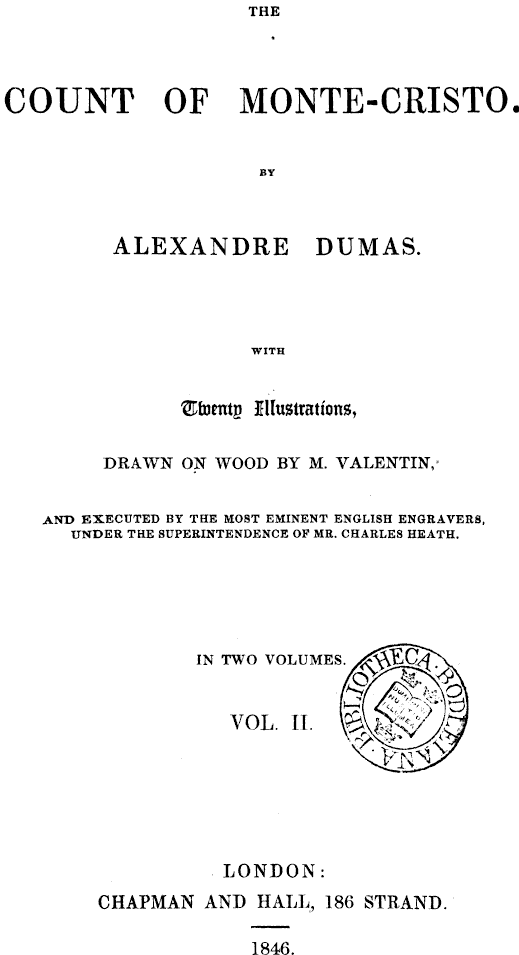
\includegraphics[height=3in]{translation/monte-cristo-english-title}

\end{frame}

\begin{frame}
  \frametitle{Machine learning for translation (google translate)}

  
  Want: $f$(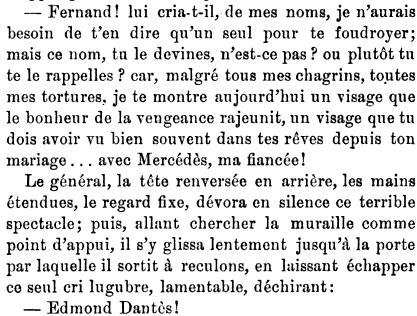
\includegraphics[width=0.5\textwidth]{translation/monte-cristo-french}) =
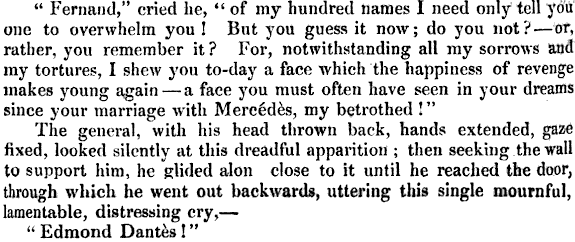
\includegraphics[width=0.8\textwidth]{translation/monte-cristo-english}

\end{frame}

\begin{frame}
  \frametitle{Machine learning for translation (google translate)}

  --- Fernand! lui cria-t-il, de mes noms, je n'aurais besoin de t'en
  dire qu'un seul pour te foudroyer; mais ce nom, tu le devines,
  n'est-ce pas ? ou plutôt tu te le rappelles ? car, malgré tous mes
  chagrins, toutes mes tortures, je te montre aujourd'hui un visage
  que le bonheur de la vengeance rajeunit, un visage que tu dois avoir
  vu bien souvent dans tes rêves depuis ton mariage ... avec Mercédès,
  ma fiancée!

  Le général, la tête renversée en arrière, les mains étendues, le
  regard fixe, dévora en silence ce terrible spectacle; puis, allant
  chercher la muraille comme point d'appui, il s'y glissa lentement
  jusqu'à la porte par laquelle il sortit à reculons, en laissant
  échapper ce seul cri lugubre, lamentable, déchirant:

  --- Edmond Dantès!

\end{frame}

\begin{frame}
  \frametitle{Machine learning for translation (google translate)}
  
  ``Fernand,'' cried he, ``of my hundred names I need only tell you
  one to overwhelm you! But you guess it now; do you not? --- or,
  rather, you remember it? For, notwithstanding all my sorrows and my
  tortures, I show you to-day a face which the happiness of revenge
  makes young again --- a face you must often have seen in your dreams
  since your marriage with Mercédès, my betrothed!''
  
  The general, with his head thrown back, hands extended, gaze fixed,
  looked silently at this dreadful apparition; then seeking the wall
  to support him, he glided along close to it until he reached the
  door, through which he went out backwards, uttering this single
  mournful, lamentable, distressing cry,---
  
  ``Edmond Dantès!''

\end{frame}



\begin{frame}
  \frametitle{Machine learning for music transcription}

  \begin{itemize}
   \item Want: $f$(mp3 file)=score for all instruments playing, e.g.
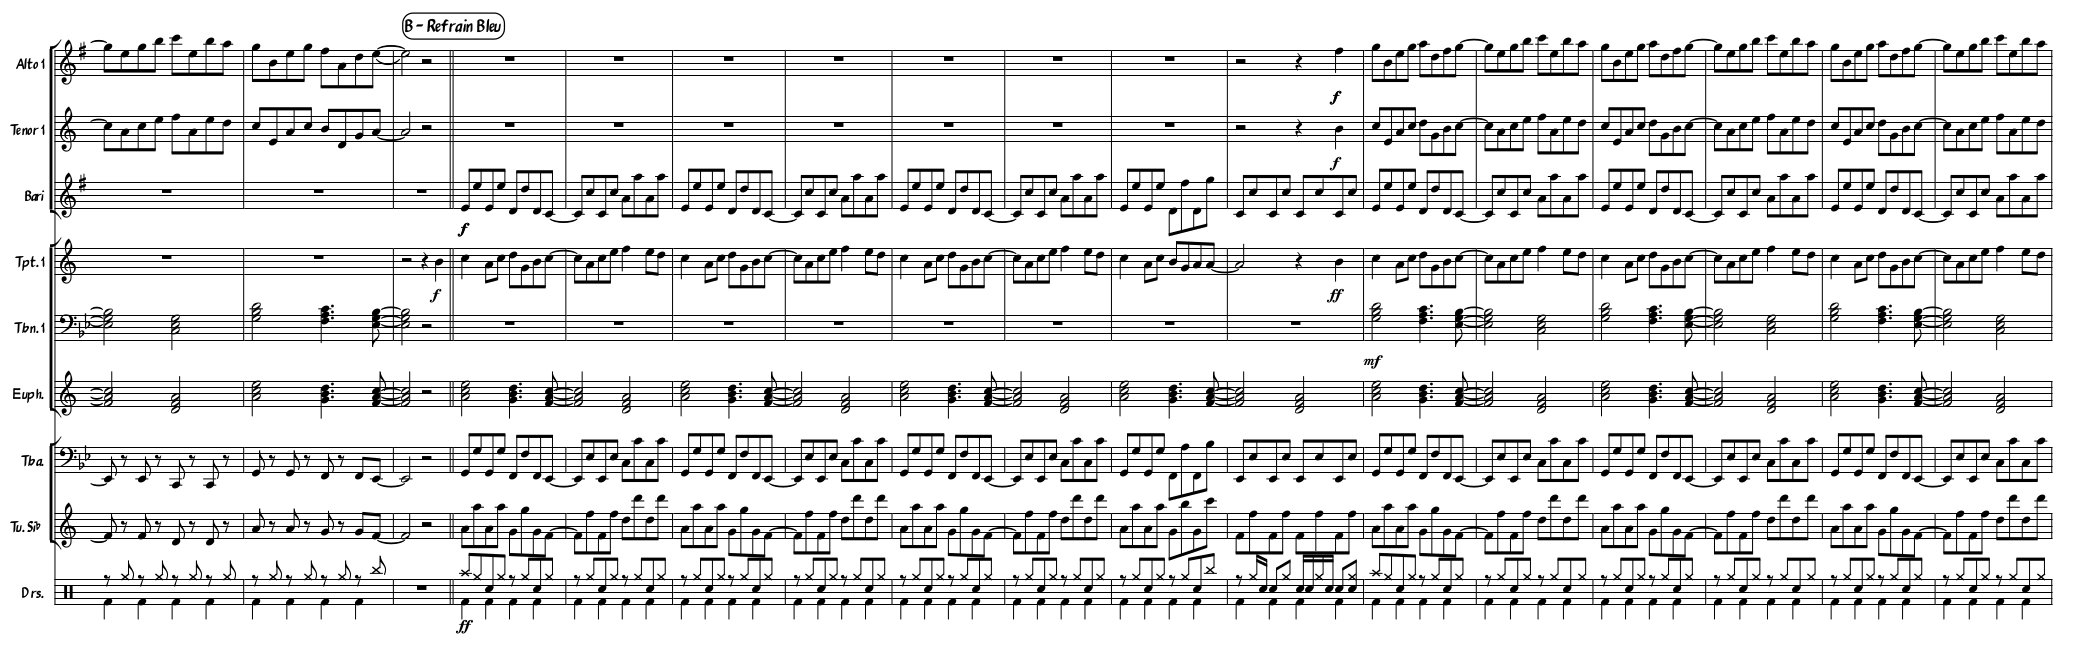
\includegraphics[width=\textwidth]{music-transcription/BFD-page2}
\item Listening to mp3 then writing score is difficult! (but possible)
\item Generating a real/recorded mp3 file based on score is also difficult
  (need skilled musicians to read/play).
\item Easy to compute \textsc{Synth}(score)=synthesized mp3 file.
\item Q: can we use synthesized mp3 files to train a ML algo?
\item  Listen to MP3s: recorded, synthesized.
  \end{itemize}
\end{frame}

\begin{frame}
  \frametitle{Machine learning for recognizing cursive handwriting}

Optical/intelligent character/word recognition 

Want: $f$(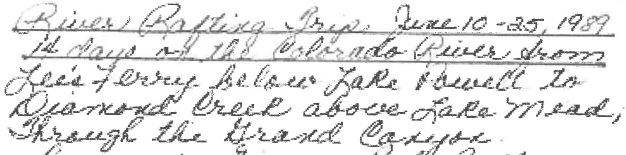
\includegraphics[width=0.9\textwidth]{grandma-handwriting/grand-canyon-page1-paragraph1})=

\only<2>{\underline{River Rafting Trip June 10--25, 1989}\\
  \underline{14 days on the Colorado River from}\\
  Lee's Ferry below Lake Powell to\\
  Diamond Creek above Lake Mead,\\
  Through the Grand Canyon}

\end{frame}

\begin{frame}
  \frametitle{Machine learning for recognizing cursive handwriting}

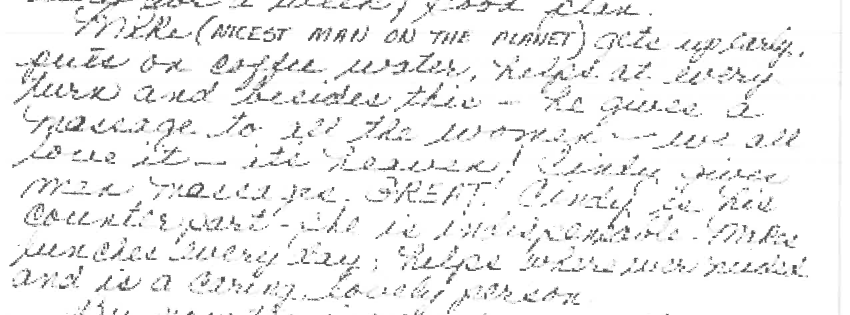
\includegraphics[width=1\textwidth]{grandma-handwriting/grand-canyon-page7}

Q: sometimes you hear about ``AI more accurate than human'' -- what
does that mean, if the human is defining the labels? 

Q: Can AI be more accurate at reading this than my grandmother, who
wrote it?

\end{frame}

\begin{frame}
  \frametitle{Machine learning for medical diagnosis}

\parbox{0.49\textwidth}{
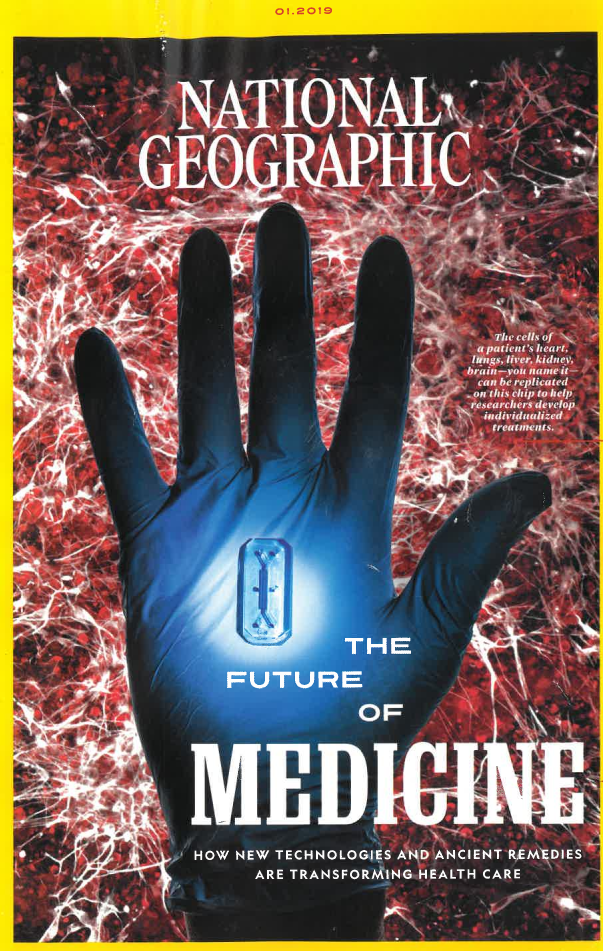
\includegraphics[height=0.9\textheight]{retinal-scans/national-geographic-medicine-cover}
}
\parbox{0.49\textwidth}{
f(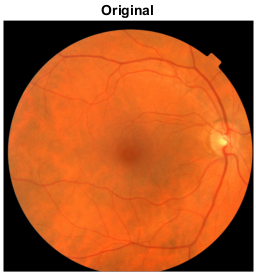
\includegraphics[width=0.5\textwidth]{retinal-scans/national-geographic-medicine-retina})=
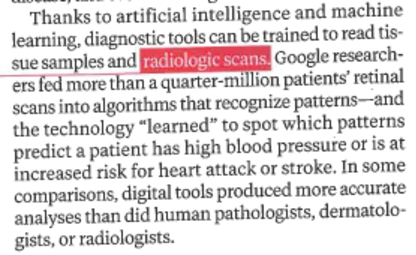
\includegraphics[width=0.5\textwidth]{retinal-scans/national-geographic-medicine-paragraph})
}

\end{frame}

\begin{frame}
  \frametitle{Machine learning for medical diagnosis 2}

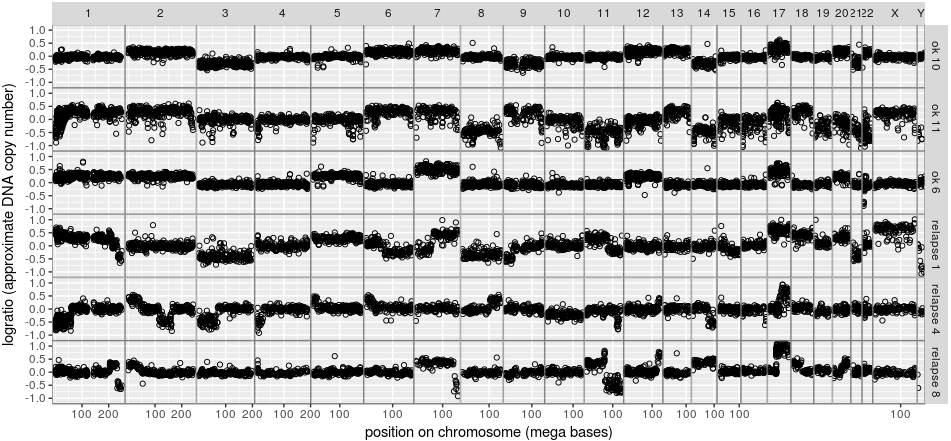
\includegraphics[width=\textwidth]{neuroblastoma-ok-relapse}

\begin{itemize}
\item Each row is a genomic profile from a cancer patient.
\item Each column is a different chromosome.
\item Approximate copy number plotted against chrom position.
\item Want $f$(profile)$\in\{\text{ok},\text{relapse}\}$.
\item Can you determine an $f$ by visual inspection?
\end{itemize}

\end{frame}


\begin{frame}
  \frametitle{Machine learning for other applications}

  I have mostly presented machine learning applications which I
  believe are good for the future of humanity. (e.g. google translate
  makes it easier for people to communicate/understand each other)

  \vskip 1in

  Q: what are some other applications of machine learning which are
  good/bad for the future of humanity? Why?

\end{frame}




\end{document}

 